% Options for packages loaded elsewhere
% Options for packages loaded elsewhere
\PassOptionsToPackage{unicode}{hyperref}
\PassOptionsToPackage{hyphens}{url}
\PassOptionsToPackage{dvipsnames,svgnames,x11names}{xcolor}
%
\documentclass[
  letterpaper,
  DIV=11,
  numbers=noendperiod]{scrreprt}
\usepackage{xcolor}
\usepackage{amsmath,amssymb}
\setcounter{secnumdepth}{5}
\usepackage{iftex}
\ifPDFTeX
  \usepackage[T1]{fontenc}
  \usepackage[utf8]{inputenc}
  \usepackage{textcomp} % provide euro and other symbols
\else % if luatex or xetex
  \usepackage{unicode-math} % this also loads fontspec
  \defaultfontfeatures{Scale=MatchLowercase}
  \defaultfontfeatures[\rmfamily]{Ligatures=TeX,Scale=1}
\fi
\usepackage{lmodern}
\ifPDFTeX\else
  % xetex/luatex font selection
\fi
% Use upquote if available, for straight quotes in verbatim environments
\IfFileExists{upquote.sty}{\usepackage{upquote}}{}
\IfFileExists{microtype.sty}{% use microtype if available
  \usepackage[]{microtype}
  \UseMicrotypeSet[protrusion]{basicmath} % disable protrusion for tt fonts
}{}
\makeatletter
\@ifundefined{KOMAClassName}{% if non-KOMA class
  \IfFileExists{parskip.sty}{%
    \usepackage{parskip}
  }{% else
    \setlength{\parindent}{0pt}
    \setlength{\parskip}{6pt plus 2pt minus 1pt}}
}{% if KOMA class
  \KOMAoptions{parskip=half}}
\makeatother
% Make \paragraph and \subparagraph free-standing
\makeatletter
\ifx\paragraph\undefined\else
  \let\oldparagraph\paragraph
  \renewcommand{\paragraph}{
    \@ifstar
      \xxxParagraphStar
      \xxxParagraphNoStar
  }
  \newcommand{\xxxParagraphStar}[1]{\oldparagraph*{#1}\mbox{}}
  \newcommand{\xxxParagraphNoStar}[1]{\oldparagraph{#1}\mbox{}}
\fi
\ifx\subparagraph\undefined\else
  \let\oldsubparagraph\subparagraph
  \renewcommand{\subparagraph}{
    \@ifstar
      \xxxSubParagraphStar
      \xxxSubParagraphNoStar
  }
  \newcommand{\xxxSubParagraphStar}[1]{\oldsubparagraph*{#1}\mbox{}}
  \newcommand{\xxxSubParagraphNoStar}[1]{\oldsubparagraph{#1}\mbox{}}
\fi
\makeatother


\usepackage{longtable,booktabs,array}
\usepackage{calc} % for calculating minipage widths
% Correct order of tables after \paragraph or \subparagraph
\usepackage{etoolbox}
\makeatletter
\patchcmd\longtable{\par}{\if@noskipsec\mbox{}\fi\par}{}{}
\makeatother
% Allow footnotes in longtable head/foot
\IfFileExists{footnotehyper.sty}{\usepackage{footnotehyper}}{\usepackage{footnote}}
\makesavenoteenv{longtable}
\usepackage{graphicx}
\makeatletter
\newsavebox\pandoc@box
\newcommand*\pandocbounded[1]{% scales image to fit in text height/width
  \sbox\pandoc@box{#1}%
  \Gscale@div\@tempa{\textheight}{\dimexpr\ht\pandoc@box+\dp\pandoc@box\relax}%
  \Gscale@div\@tempb{\linewidth}{\wd\pandoc@box}%
  \ifdim\@tempb\p@<\@tempa\p@\let\@tempa\@tempb\fi% select the smaller of both
  \ifdim\@tempa\p@<\p@\scalebox{\@tempa}{\usebox\pandoc@box}%
  \else\usebox{\pandoc@box}%
  \fi%
}
% Set default figure placement to htbp
\def\fps@figure{htbp}
\makeatother





\setlength{\emergencystretch}{3em} % prevent overfull lines

\providecommand{\tightlist}{%
  \setlength{\itemsep}{0pt}\setlength{\parskip}{0pt}}



 


\KOMAoption{captions}{tableheading}
\makeatletter
\@ifpackageloaded{bookmark}{}{\usepackage{bookmark}}
\makeatother
\makeatletter
\@ifpackageloaded{caption}{}{\usepackage{caption}}
\AtBeginDocument{%
\ifdefined\contentsname
  \renewcommand*\contentsname{Table of contents}
\else
  \newcommand\contentsname{Table of contents}
\fi
\ifdefined\listfigurename
  \renewcommand*\listfigurename{List of Figures}
\else
  \newcommand\listfigurename{List of Figures}
\fi
\ifdefined\listtablename
  \renewcommand*\listtablename{List of Tables}
\else
  \newcommand\listtablename{List of Tables}
\fi
\ifdefined\figurename
  \renewcommand*\figurename{Figure}
\else
  \newcommand\figurename{Figure}
\fi
\ifdefined\tablename
  \renewcommand*\tablename{Table}
\else
  \newcommand\tablename{Table}
\fi
}
\@ifpackageloaded{float}{}{\usepackage{float}}
\floatstyle{ruled}
\@ifundefined{c@chapter}{\newfloat{codelisting}{h}{lop}}{\newfloat{codelisting}{h}{lop}[chapter]}
\floatname{codelisting}{Listing}
\newcommand*\listoflistings{\listof{codelisting}{List of Listings}}
\makeatother
\makeatletter
\makeatother
\makeatletter
\@ifpackageloaded{caption}{}{\usepackage{caption}}
\@ifpackageloaded{subcaption}{}{\usepackage{subcaption}}
\makeatother
\usepackage{bookmark}
\IfFileExists{xurl.sty}{\usepackage{xurl}}{} % add URL line breaks if available
\urlstyle{same}
\hypersetup{
  pdftitle={Muhammad Farrel Wibowo},
  pdfauthor={13523153 Muhammad Farrel Wibowo},
  colorlinks=true,
  linkcolor={blue},
  filecolor={Maroon},
  citecolor={Blue},
  urlcolor={Blue},
  pdfcreator={LaTeX via pandoc}}


\title{Muhammad Farrel Wibowo}
\usepackage{etoolbox}
\makeatletter
\providecommand{\subtitle}[1]{% add subtitle to \maketitle
  \apptocmd{\@title}{\par {\large #1 \par}}{}{}
}
\makeatother
\subtitle{Portfolio Asesmen II-2100 KIPP}
\author{13523153 Muhammad Farrel Wibowo}
\date{2027-07-10}
\begin{document}
\maketitle

\renewcommand*\contentsname{Table of contents}
{
\hypersetup{linkcolor=}
\setcounter{tocdepth}{2}
\tableofcontents
}

\bookmarksetup{startatroot}

\chapter*{Selamat Berjumpa}\label{selamat-berjumpa}
\addcontentsline{toc}{chapter}{Selamat Berjumpa}

\markboth{Selamat Berjumpa}{Selamat Berjumpa}

\begin{figure}[H]

{\centering \includegraphics[width=9.5\linewidth,height=\textheight,keepaspectratio]{../images/profile-pict.jpeg}

}

\caption{About Me}

\end{figure}%

Muhammad Farrel Wibowo adalah mahasiswa Teknik Informatika Institut
Teknologi Bandung angkatan 2023. Lahir di Jakarta pada 18 Juni 2005,
kini menetap di Jatinangor untuk menjalani aktivitas perkuliahan,
sementara rumah keluarganya masih berada di Jakarta. Sejak kecil Farrel
sudah akrab dengan dunia teknologi---mulai dari smartphone, komputer,
hingga internet---yang menumbuhkan rasa ingin tahu tentang bagaimana
teknologi bekerja dan bagaimana ia dapat mengubah kehidupan manusia.

Sehari-hari, Farrel dikenal sebagai sosok yang disiplin, pekerja keras,
dan reflektif. Ia memiliki berbagai hobi seperti olahraga gym,
fotografi, otomotif, videografi, dan tenis. Namun di balik banyaknya
minat tersebut, benang merah yang mengikat semuanya adalah rasa ingin
belajar dan berkembang secara berkelanjutan.

\bookmarksetup{startatroot}

\chapter{UTS-1 All About Me}\label{uts-1-all-about-me}

\begin{figure}[H]

{\centering \includegraphics[width=9.5\linewidth,height=\textheight,keepaspectratio]{All_About_me/../images/profile-pict.jpeg}

}

\caption{About Me}

\end{figure}%

``Tahun itu saya duduk di depan laptop dengan ekspresi antara pasrah dan
penasaran---mirip wajah mahasiswa yang menunggu nilai akhir di KRS.
Layar menampilkan dua kata yang sukses bikin jantung pindah ke
tenggorokan: \textbf{`Tidak Lulus.'}\\
Bukannya menangis, saya malah membuka YouTube dan menonton video
motivasi---yang ironisnya diawali iklan \emph{Shopee Payday Sale}. Tapi
justru dari situ saya sadar: hidup bukan soal jalur SNBT atau Mandiri,
tapi soal siapa yang paling tahan saat server penuh.''

Hai, saya \textbf{Muhammad Farrel Wibowo}, mahasiswa \textbf{Teknik
Informatika ITB 2023}.\\
Lahir di Jakarta, besar di antara kabel charger yang hilang dan update
Windows yang tak berkesudahan. Kini saya tinggal di Jatinangor---tempat
di mana kopi dan Wi-Fi menjadi dua sumber energi utama.\\
Teknologi bagi saya bukan sekadar perangkat keras dan kode, tapi juga
\emph{teman ngobrol} yang tidak pernah bosan mendengarkan \emph{error
log} saya.

\section{\texorpdfstring{\textbf{Kisah yang Membentuk Diri Anda:
Mengenal Kekuatan Identitas
Naratif}}{Kisah yang Membentuk Diri Anda: Mengenal Kekuatan Identitas Naratif}}\label{kisah-yang-membentuk-diri-anda-mengenal-kekuatan-identitas-naratif}

Saya tumbuh dengan rasa ingin tahu yang agak berlebihan terhadap hal-hal
teknis: bagaimana mesin cuci bisa berhenti sendiri, kenapa \emph{loading
bar} selalu berhenti di 99\%, dan kenapa printer selalu rusak saat
deadline.\\
Di \textbf{MAN 4 Jakarta}, saya belajar menggabungkan logika dengan
kreativitas---bergabung di klub robotika dan teknologi informasi.\\
Puncaknya, tim kami mendapat medali perak di \textbf{AISEF} berkat
proyek \emph{Early Warning Flood System}.\\
Saat itu saya sadar: teknologi bukan sekadar ``keren'', tapi juga bisa
mencegah orang telat kabur dari banjir---itulah versi saya dari
\emph{superhero moment.}

\subsection{\texorpdfstring{\textbf{1. Tiga Lapisan Diri Anda: Di Mana
Cerita Hidup Anda
Berada?}}{1. Tiga Lapisan Diri Anda: Di Mana Cerita Hidup Anda Berada?}}\label{tiga-lapisan-diri-anda-di-mana-cerita-hidup-anda-berada}

Mengikuti kerangka dari Dan P. McAdams, saya bisa memetakan perjalanan
diri saya sebagai berikut:

\begin{longtable}[]{@{}
  >{\raggedright\arraybackslash}p{(\linewidth - 4\tabcolsep) * \real{0.2258}}
  >{\raggedright\arraybackslash}p{(\linewidth - 4\tabcolsep) * \real{0.3871}}
  >{\raggedright\arraybackslash}p{(\linewidth - 4\tabcolsep) * \real{0.3871}}@{}}
\toprule\noalign{}
\begin{minipage}[b]{\linewidth}\raggedright
Level
\end{minipage} & \begin{minipage}[b]{\linewidth}\raggedright
Deskripsi
\end{minipage} & \begin{minipage}[b]{\linewidth}\raggedright
Debug Note
\end{minipage} \\
\midrule\noalign{}
\endhead
\bottomrule\noalign{}
\endlastfoot
\textbf{1. Traits (Sifat Dasar)} & Disiplin, logis, reflektif. Kadang
terlalu serius. & \emph{Work in progress: belajar bercanda tanpa
menimbulkan bug percakapan.} \\
\textbf{2. Personal Concern} & Menghargai proses dan kegigihan; melihat
gagal sebagai ``versi beta dari sukses.'' & \emph{Masalah muncul jika
versi beta ini terlalu sering di-update tanpa tidur cukup.} \\
\textbf{3. Narrative Identity} & Melihat hidup sebagai proyek open
source: terbuka untuk kontribusi dan perbaikan. & \emph{Merge request
selalu diterima asal disertai niat baik.} \\
\end{longtable}

Kegagalan SNBT jadi \emph{milestone bugfix} pertama saya. Jalur Mandiri
ke ITB bukan rute darurat, tapi pembuktian bahwa kadang \emph{error 404}
berarti ``Opportunity Not Found---Yet.''

\subsection{\texorpdfstring{\textbf{2. Pola-Pola Kisah Kehidupan: Apa
yang Membuat Sebuah Cerita
Bermanfaat?}}{2. Pola-Pola Kisah Kehidupan: Apa yang Membuat Sebuah Cerita Bermanfaat?}}\label{pola-pola-kisah-kehidupan-apa-yang-membuat-sebuah-cerita-bermanfaat}

Cerita hidup saya mencerminkan pola penebusan (redemption)---dari
kegagalan menuju keberhasilan, dari keterbatasan menuju kesempatan baru.
Kegagalan masuk kampus favorit bukan akhir cerita, tetapi bab pembuka
dari narasi yang lebih bermakna. Kini, setelah menjadi mahasiswa, saya
juga mulai mengembangkan pola agensi dan koneksi, di mana peran saya
tidak lagi sebatas individu yang berjuang, tetapi bagian dari ekosistem
yang saling tumbuh bersama.

\begin{longtable}[]{@{}
  >{\raggedright\arraybackslash}p{(\linewidth - 2\tabcolsep) * \real{0.2000}}
  >{\raggedright\arraybackslash}p{(\linewidth - 2\tabcolsep) * \real{0.8000}}@{}}
\toprule\noalign{}
\begin{minipage}[b]{\linewidth}\raggedright
Pola
\end{minipage} & \begin{minipage}[b]{\linewidth}\raggedright
Dampak \& Pembelajaran
\end{minipage} \\
\midrule\noalign{}
\endhead
\bottomrule\noalign{}
\endlastfoot
\textbf{Penebusan (Negatif → Positif)} & Dari gagal SNBT ke lulus ITB
lewat jalur Mandiri. Belajar sabar menunggu hasil bukan cuma di website
pendaftaran tapi juga dalam hidup. \\
\textbf{Agensi (Aktor Efektif)} & Menjadi mentor TEC, ikut hackathon,
dan belajar bahwa tim kuat bukan yang tak pernah debat, tapi yang bisa
debat tanpa uninstall Discord. \\
\textbf{Koneksi (Rasa Memiliki)} & Di HMIF dan ITB Jazz, saya menemukan
bahwa irama kerja tim sama pentingnya dengan harmoni musik. \\
\textbf{Momen Berkilau} & Juara 3 Hackathon pertama: kombinasi antara
\emph{panic coding} dan \emph{coffee overdose} yang ternyata efektif. \\
\end{longtable}

\subsection{\texorpdfstring{\textbf{3. Seni Memberi Makna: Kekuatan
Super Anda dalam
Bernalar}}{3. Seni Memberi Makna: Kekuatan Super Anda dalam Bernalar}}\label{seni-memberi-makna-kekuatan-super-anda-dalam-bernalar}

Saya belajar bahwa kesalahan bukan musuh, tapi \emph{unit test} dari
semesta.\\
Ketika server crash di tengah presentasi hackathon, saya tidak
panik---saya hanya berkata, ``Tenang, ini cuma simulasi stres.''\\
Bagi saya, berpikir jernih di tengah kekacauan adalah bentuk
spiritualitas versi \emph{techie}.

Hackathon itu memberi empat pelajaran hidup: 1. \textbf{Framing masalah}
lebih penting dari jumlah baris kode.\\
2. \textbf{Kolaborasi cepat} lebih efektif daripada ``brainstorming
abadi.''\\
3. \textbf{Integrasi cepat} lebih berharga dari teori sempurna.\\
4. \textbf{Storytelling produk} harus jujur; jangan jualan ``AI'' kalau
sebenarnya cuma \emph{if-else}.

Kesadaran terbesar saya: dunia ini bukan kompetisi siapa paling pintar,
tapi siapa paling konsisten memperbaiki diri tanpa kehilangan tawa.

\subsection{\texorpdfstring{\textbf{4. Mulai Menulis Ulang Kisah Anda:
Dua Langkah
Praktis}}{4. Mulai Menulis Ulang Kisah Anda: Dua Langkah Praktis}}\label{mulai-menulis-ulang-kisah-anda-dua-langkah-praktis}

\begin{enumerate}
\def\labelenumi{\arabic{enumi}.}
\item
  \textbf{Eksternalisasi Masalah:}\\
  Saya berhenti berkata ``saya gagal,'' dan mulai berkata ``program saya
  sedang \emph{buggy}.''\\
  Versi ini lebih ringan di hati dan lebih mudah diperbaiki.
\item
  \textbf{Temukan Momen Berkilau:}\\
  Saat lupa makan karena ngoding dan sadar jam sudah menunjukkan pukul 3
  pagi---itu bukan lelah, itu \emph{flow state} (katanya).
\end{enumerate}

\subsection{\texorpdfstring{\textbf{5. Kesimpulan: Kisah Saya Masih
Terus
Ditulis}}{5. Kesimpulan: Kisah Saya Masih Terus Ditulis}}\label{kesimpulan-kisah-saya-masih-terus-ditulis}

Saya tidak tahu ke mana repositori hidup saya akan \emph{push}
selanjutnya, tapi saya tahu setiap \emph{commit}---entah sukses atau
gagal---adalah bagian dari versi terbaik diri saya yang terus
diperbarui.\\
Teknologi hanyalah alat; manusia adalah algoritma yang belajar dari
empati.\\
Dan saya? Masih di tahap \emph{debugging life}, tapi kali ini dengan
\emph{humor log} yang aktif.

\bookmarksetup{startatroot}

\chapter{UTS-2 My Songs for You}\label{uts-2-my-songs-for-you}

Dari Hati Performed by

Club Eighties

\url{https://youtu.be/USF8xr4QEa0?si=tu8tP-XTlD5Bz-b9}

\subsubsection{Makna dan Alasan Pemilihan
Lagu}\label{makna-dan-alasan-pemilihan-lagu}

Saya memilih lagu \textbf{``Dari Hati''} bukan hanya karena nadanya enak
didengar saat hujan turun sambil ngoding, tapi karena liriknya punya
\emph{debug power} tersendiri: bisa menenangkan pikiran yang sedang
\emph{syntax error} karena cinta.\\
Lagu ini sederhana, jujur, dan tidak berusaha jadi romantis berlebihan.
Ia berbicara tentang kejujuran dan kerentanan --- sesuatu yang sering
kita hindari, terutama kalau kamu tipe orang yang bilang ``nggak apa-apa
kok'' padahal tab browser sudah penuh lirik galau.

Bait \emph{``Ku ingin jujur apa adanya, dari hati''} jadi refleksi
tentang bagaimana mencintai tanpa kode rahasia: tidak perlu
\texttt{if-else}, cukup \texttt{return\ honesty;}.\\
Itulah yang membuat saya jatuh cinta pada lagu ini --- ia menulis ulang
cinta dengan bahasa manusia, bukan algoritma.

\subsection{Lirik Lagunya}\label{lirik-lagunya}

{[}Intro{]} Andai engkau tahu Bila menjadi aku, sejuta rasa di hati Lama
tlah kupendam Tapi akan kucoba mengatakannya

{[}Verse 1{]} Ku ingin kau menjadi milikku Entah bagaimana caranya
Lihatlah mataku untuk memintamu Ku ingin jalani bersamamu Coba dengan
sepenuh hati Ku ingin jujur apa adanya Dari hati

{[}Chorus 1{]} Kini engkau tahu aku menginginkanmu Tapi takkan
kupaksakan Dan kupastikan kau belahan hati Bila milikku oooo Ku ingin
kau menjadi milikku Entah bagaimana caranya Lihatlah mataku untuk
memintamu Aku ingin jalani bersamamu Coba dengan sepenuh hati Ku ingin
jujur apa adanya

{[}Bridge{]} Menarilah bersamaku Dengan bintang-bintang Sambutlah diriku
Untuk memelukmu

{[}Chorus 2{]} Ku ingin kau menjadi milikku Entah bagaimana caranya
Lihatlah mataku untuk memintamu Ku ingin jalani bersamamu Coba dengan
sepenuh hati Ku ingin jujur apa adanya Dari hati

{[}Outro{]} Dari hati

\subsection{Narasi Personal}\label{narasi-personal}

Saya pertama kali mendengar lagu ini bukan di konser, bukan juga dari
playlist Spotify, tapi dari \textbf{speaker kantin kampus} yang
kualitasnya lebih mirip toa masjid yang pensiun dini.\\
Tapi entah kenapa, di tengah suara gorengan, sendok jatuh, dan
teman-teman debat soal tugas, liriknya menembus semua kebisingan itu.

\begin{quote}
\emph{``Ku ingin jujur apa adanya, dari hati.''}
\end{quote}

Kalimat itu seperti pesan error yang sulit di-\emph{ignore}.\\
Saya yang biasanya logis, tiba-tiba merasa dipanggil untuk berhenti
berpura-pura kuat.\\
Selama ini saya pikir mencintai itu tentang memiliki; ternyata, seperti
coding, yang penting bukan siapa yang menjalankan, tapi siapa yang tetap
\emph{maintain} meski sering crash.

Lagu ini lucunya ikut hadir di berbagai fase absurd hidup saya: - Saat
skripsi mini kacau dan saya mengganti \texttt{SELECT\ *\ FROM} dengan
\texttt{SELECT\ *\ FROM\ hati;} - Saat ngopi jam 2 pagi sambil menatap
\emph{deadline} yang lebih dingin dari kopi itu sendiri. - Saat sadar
bahwa ``jujur'' bukan berarti harus benar terus, tapi berani mengakui
ketika salah.

Lagu ini bukan sekadar lagu cinta --- ini reminder agar saya tetap jujur
pada proses hidup, entah dalam hubungan atau proyek kelompok yang
server-nya down.

\begin{center}\rule{0.5\linewidth}{0.5pt}\end{center}

\subsection{\texorpdfstring{Karya Respon: \emph{Puisi
Pendek}}{Karya Respon: Puisi Pendek}}\label{karya-respon-puisi-pendek}

\begin{quote}
Tak semua cinta butuh jawaban,\\
kadang cukup dieksekusi tanpa \texttt{WHERE} atau \texttt{LIMIT}.

Hati bukan database, tapi tetap butuh \emph{commit} agar tak kehilangan
jejak.

``Dari hati,'' katanya,\\
dan aku percaya ---\\
bahkan kode yang paling sederhana pun\\
bisa menjalankan cinta yang paling tulus.
\end{quote}

\begin{center}\rule{0.5\linewidth}{0.5pt}\end{center}

\subsection{💭 Refleksi}\label{refleksi}

``Dari Hati'' mengingatkan saya bahwa ketulusan adalah logika paling
irasional yang pernah ada --- tidak bisa di-\emph{compile}, tapi bisa
dirasakan.\\
Ia mengajarkan bahwa memberi tanpa mengharap balasan bukanlah kelemahan,
tapi bentuk tertinggi dari kesadaran diri.\\
Ketika saya mendengar lagu ini hari ini, saya tidak lagi berpikir
tentang siapa yang akan saya cintai nanti, tapi \emph{bagaimana caranya
saya bisa tetap mencintai dengan jujur} --- baik kepada orang lain,
pekerjaan, maupun diri sendiri.

\begin{center}\rule{0.5\linewidth}{0.5pt}\end{center}

\bookmarksetup{startatroot}

\chapter{UTS-3 My Stories for You}\label{uts-3-my-stories-for-you}

\section{\texorpdfstring{\textbf{Sebuah Kisah: ``Belajar Menemukan Diri
di Tengah
Perjalanan''}}{Sebuah Kisah: ``Belajar Menemukan Diri di Tengah Perjalanan''}}\label{sebuah-kisah-belajar-menemukan-diri-di-tengah-perjalanan}

Hidup saya bukan rangkaian kemenangan, melainkan rangkaian proses
memahami arti kegagalan, kesabaran, dan keyakinan. Setiap langkah kecil
membawa pelajaran baru---dan kisah inilah yang ingin saya bagikan, bukan
karena sempurna, tetapi karena ia jujur dan membentuk siapa saya
sekarang.

\begin{center}\rule{0.5\linewidth}{0.5pt}\end{center}

\subsection{\texorpdfstring{\textbf{Awal
Perjalanan}}{Awal Perjalanan}}\label{awal-perjalanan}

Saya tumbuh sebagai anak yang selalu penasaran pada teknologi. Dari
komputer, internet, hingga robotik di SMA, semua itu membuat saya kagum
pada bagaimana sesuatu bisa ``hidup'' karena logika dan kode. Namun di
balik rasa ingin tahu itu, saya sering merasa belum cukup baik. Saya
takut gagal, takut tidak memenuhi ekspektasi.

Kegagalan pertama besar yang saya rasakan adalah saat tidak lolos
\textbf{SNBT}, ujian masuk perguruan tinggi yang selama ini saya
harapkan. Hari itu saya merasa dunia berhenti. Tetapi justru di titik
itu saya belajar makna \emph{penebusan}. Saya belajar bahwa hidup tidak
selalu harus berjalan lurus; kadang kita harus tersesat dulu untuk
benar-benar menemukan arah. Saya memutuskan mencoba jalur
\textbf{Mandiri ITB}, dan berhasil diterima di jurusan impian saya:
\textbf{Teknik Informatika Institut Teknologi Bandung}.

Sejak saat itu, saya memahami bahwa kegagalan bukan akhir cerita---ia
hanyalah tanda bahwa saya sedang ditulis ulang menjadi versi diri yang
lebih baik.

\begin{center}\rule{0.5\linewidth}{0.5pt}\end{center}

\subsection{\texorpdfstring{\textbf{Proses dan
Pembelajaran}}{Proses dan Pembelajaran}}\label{proses-dan-pembelajaran}

Perkuliahan di ITB bukan hanya tentang memahami algoritma atau teori,
tapi tentang membangun daya tahan mental. Di sinilah saya belajar
pentingnya keseimbangan antara ambisi dan empati.\\
Saya belajar menata waktu, menahan ego, menerima perbedaan cara
berpikir, dan memahami bahwa kesuksesan kolektif sering kali lebih
bermakna daripada kemenangan pribadi.

Puncak pengalaman itu datang ketika tim saya meraih \textbf{Juara 3
Hackathon pertama saya di bangku kuliah}.\\
Lomba itu bukan sekadar kompetisi, tapi ujian nyata tentang bagaimana
sebuah ide bisa diwujudkan di bawah tekanan waktu dan perbedaan
pendapat. Saya belajar banyak hal:\\
- Bahwa komunikasi adalah inti dari kolaborasi.\\
- Bahwa keputusan kecil, seperti siapa yang menulis kode terakhir atau
siapa yang mempresentasikan produk, bisa menentukan keberhasilan
bersama.\\
- Bahwa ketenangan dan rasa saling percaya lebih berharga daripada
kecepatan.

Sejak hari itu, saya menyadari bahwa kompetisi sejati bukan antara saya
dan orang lain---melainkan antara saya dan versi diri saya kemarin.

\begin{center}\rule{0.5\linewidth}{0.5pt}\end{center}

\subsection{\texorpdfstring{\textbf{Makna dan Inspirasi untuk Orang
Lain}}{Makna dan Inspirasi untuk Orang Lain}}\label{makna-dan-inspirasi-untuk-orang-lain}

Dari setiap perjalanan itu, saya ingin membagikan satu pesan
sederhana:\\
\textgreater{} ``Hidup tidak akan selalu berjalan sesuai rencana, tetapi
rencana Tuhan selalu berjalan sesuai kebutuhan kita.''

Kegagalan, kehilangan, bahkan ketidakpastian, semuanya adalah ruang
belajar untuk menemukan siapa diri kita sebenarnya.\\
Saya percaya bahwa setiap orang punya cerita yang bisa menyembuhkan
orang lain.\\
Dan jika kisah saya bisa membuat satu orang saja merasa lebih kuat untuk
bangkit, maka perjalanan ini sudah cukup berarti.

\begin{center}\rule{0.5\linewidth}{0.5pt}\end{center}

\subsection{\texorpdfstring{\textbf{Penutup: My Stories for
You}}{Penutup: My Stories for You}}\label{penutup-my-stories-for-you}

Lagu \emph{``Dari Hati''} yang saya pilih di tugas sebelumnya dan kisah
ini memiliki benang merah yang sama---\emph{kejujuran.}\\
Baik dalam cinta maupun dalam hidup, hanya kejujuran yang mampu menuntun
kita pada makna sejati.

Maka ``My Stories for You'' bukan hanya cerita tentang saya,\\
tetapi tentang keberanian untuk tetap percaya,\\
tentang proses menemukan arah di tengah ketidakpastian,\\
dan tentang bagaimana setiap kegagalan dapat berubah menjadi awal dari
sesuatu yang indah---\\
selama dijalani \textbf{dari hati.}

\bookmarksetup{startatroot}

\chapter{UTS-4 My SHAPE (Spiritual Gifts, Heart, Abilities, Personality,
Experiences)}\label{uts-4-my-shape-spiritual-gifts-heart-abilities-personality-experiences}

\begin{quote}
\textbf{Tujuan:} Merangkum rancangan diri (charter) agar saya melayani,
berkarya, dan memimpin secara paling selaras dengan karunia dan
pengalaman hidup saya. Dapat langsung ditempel ke halaman \textbf{UTS-4
--- My SHAPE} dan dipakai sebagai acuan aksi 90 hari.
\end{quote}

\section{\texorpdfstring{Sumber
\href{StrengthsProfile-Muhammad-Farrel.pdf}{VIA
assessment}}{Sumber VIA assessment}}\label{sumber-via-assessment}

\section{0) Ringkasan 1 Halaman}\label{ringkasan-1-halaman}

\textbf{Peran Inti:} Builder--Mentor Technologist --- pembuat solusi
nyata berbasis software/hardware yang tumbuh lewat kolaborasi, lalu
membagikannya ke komunitas (teman seangkatan, adik tingkat, dan
komunitas kampus). \textbf{Misi:} Mengubah rasa ingin tahu menjadi karya
yang bermanfaat---menghadirkan produk kecil yang memecahkan masalah
nyata, sambil membangun diri dan orang lain (belajar bersama, saling
dorong). \textbf{Kekuatan Utama:} disiplin \& ketekunan, kejujuran,
sense of fairness \& tim, kepemimpinan kolaboratif, pertimbangan logis,
harapan \& antusiasme, product thinking cepat. (dikonfirmasi oleh VIA:
Spiritualitas, Keadilan, Pertimbangan, Kepemimpinan, Kerja Tim,
Kejujuran, Kebaikan, Aturan Diri, Kasih, Ketekunan, dll.) \textbf{Dampak
yang Dituju:} mini-produk dan proyek kampus yang ship-able, kolaborasi
sehat, serta kultur belajar yang suportif (di TEC/HMIF/komunitas IF).

\textbf{Peta SHAPE (singkat):}

\begin{itemize}
\tightlist
\item
  \textbf{S --- Spiritual Gifts:} Encouragement/Exhortation, Serving,
  Leadership (kolaboratif), Teaching awal (peer tutoring).
\item
  \textbf{H --- Heart (Minat \& Cinta Pelayanan):} hands-on teknologi
  (AI/aplikasi web/IoT ringan), kompetisi \& hackathon, konten kreatif
  (foto--video), olahraga untuk disiplin diri.
\item
  \textbf{A --- Abilities (Kemampuan):}rapid prototyping (React/Next
  atau Python/Flask/FastAPI), integrasi API, Git workflow, presentasi \&
  demo storytelling, produksi konten (editing).
\item
  \textbf{P --- Personality (Gaya Kepribadian Kerja):} adil \&
  tim-oriented, reflektif-logis, jujur, disiplin, hopeful-energetic;
  nyaman memimpin saat perlu, tetap rendah hati.
\item
  \textbf{E --- Experiences (Pengalaman Kunci):}AISEF Silver (Arduino
  Wi-Fi-Blynk flood warning), klub robotik/ICT/band, Juara 3 Hackathon
  (kuliah), proyek komunitas (TEC/HMIF/ITB Jazz), hobi kreatif \&
  olahraga.
\end{itemize}

\begin{center}\rule{0.5\linewidth}{0.5pt}\end{center}

\section{1) S --- Spiritual Gifts (Karunia
Rohani)}\label{s-spiritual-gifts-karunia-rohani}

\begin{itemize}
\tightlist
\item
  \textbf{Teaching \& Wisdom/Discernment:} cenderung menguatkan tim,
  bantu rekan saat stuck, senang berbagi how-to.
\item
  \textbf{Leadership \& Administration:} menjaga kekompakan, membagi
  peran, fokus ship; cocok jadi squad lead kecil.
\item
  \textbf{Teaching (pemula/peer):} nyaman menjelaskan langkah praktis
  (setup, integrasi API, debug tactics) pada adik tingkat.
\end{itemize}

\begin{center}\rule{0.5\linewidth}{0.5pt}\end{center}

\section{2) H --- Heart (Minat, Nilai,
Kepedulian)}\label{h-heart-minat-nilai-kepedulian}

\begin{itemize}
\item
  \textbf{Teknologi praktis yang ``jadi barang'':} web/app ringan, AI
  kecil yang terasa gunanya, IoT sederhana.
\item
  \textbf{Kompetisi \& hackathon:} senang ritme cepat, scoping MVP, dan
  demo day.
\item
  \textbf{Kreativitas visual:} fotografi--videografi untuk dokumentasi
  tim/produk.
\item
  \textbf{Keseimbangan hidup:} olahraga (gym, tenis) untuk disiplin \&
  fokus.
\item
  \textbf{Nilai utama:} keadilan, kejujuran, dan team first (adil dalam
  pembagian kredit/kerja).
\end{itemize}

\textbf{Masalah yang ingin dipecahkan:}

\begin{center}\rule{0.5\linewidth}{0.5pt}\end{center}

\section{3) A --- Abilities (Kemampuan
Andal)}\label{a-abilities-kemampuan-andal}

\begin{itemize}
\item
  \textbf{Teknis:}
\item
  Rapid prototyping (frontend/backend sederhana), integrasi API, auth
  dasar, error handling seperlunya.
\item
  IoT ringan (warisan AISEF: Arduino + konektivitas), otomasi kecil.
\item
  Git branch--PR--review cepat; pitching \& live demo.
\item
  \textbf{Kreatif \& Komunikasi:} video editing, visual asset untuk
  launch/demo.
\item
  \textbf{Tim \& Eksekusi:} scoping, time-boxing, menjaga ritme stand-up
  singkat, trade-off teknis jelas.
\end{itemize}

\begin{center}\rule{0.5\linewidth}{0.5pt}\end{center}

\section{4) P --- Personality (Gaya Kerja \&
Kolaborasi)}\label{p-personality-gaya-kerja-kolaborasi}

\begin{itemize}
\item
  \textbf{Fair-team player \& collaborative leader} (suka menjaga rasa
  adil/kebersamaan).
\item
  \textbf{Reflective--logical}(pertimbangan kuat, tidak cepat
  menyimpulkan).
\item
  \textbf{Honest \& disciplined} (konsisten, bisa diandalkan).
\item
  \textbf{Hopeful-energetic} (membawa energi positif saat sprint).
\item
  \textbf{Semua selaras dengan profil VIA:} Keadilan, Pertimbangan,
  Kepemimpinan, Kerja Tim, Kejujuran, Aturan Diri, Harapan, Ketekunan,
  Kasih, Kebaikan.
\end{itemize}

\begin{center}\rule{0.5\linewidth}{0.5pt}\end{center}

\section{5) E --- Experiences (Pengalaman
Pembentuk)}\label{e-experiences-pengalaman-pembentuk}

\begin{itemize}
\item
  \textbf{AISEF Silver:} early warning flood system
  (Arduino--Wi-Fi--Blynk) → rasa ``teknologi untuk manfaat''.
\item
  \textbf{Klub robotik/ICT/band (SMA):}disiplin proyek \& panggung.
\item
  \textbf{Juara 3 Hackathon (kuliah):} framing problem, scope MVP,
  integrasi cepat, storytelling.
\item
  \textbf{Komunitas kampus (TEC/HMIF/ITB Jazz):} ruang tumbuh
  kolaborasi, peer-mentoring, eksekusi event.
\item
  \textbf{Pelajaran inti: keberhasilan} = disiplin kecil + kejujuran +
  kerja tim + keberanian ship dulu, perfect later.
\end{itemize}

\textbf{Pelajaran Inti:} integrasi iman--ilmu--nilai; sistem yang baik
melipatgandakan orang baik; narasi menggerakkan aksi.

\begin{center}\rule{0.5\linewidth}{0.5pt}\end{center}

\section{6) Piagam Diri (Self‑Charter)}\label{piagam-diri-selfcharter}

\textbf{Misi Hidup:} Menciptakan mini-produk bermanfaat dan kultur
belajar kolaboratif; tumbuh bersama komunitas lewat proyek nyata.
\textbf{Nilai Inti:} adil, jujur, disiplin, peduli, berpengharapan.
\textbf{Peran Inti:} builder (yang mengeksekusi), scoper (yang
memfokuskan), mentor sebaya. \textbf{Kompas Keputusan:} (1) manfaat
pengguna cepat terasa; (2) adil bagi tim; (3) bisa dirawat \&
ditingkatkan; (4) evidence-based; (5) etis \& transparan. \textbf{Janji
Pelayanan:} hadir tepat waktu, commit yang realistis, berbagi ilmu,
menghargai kredit tim. \textbf{Batasan:} menolak praktik curang, scope
di luar kapasitas realistis, dan proyek tanpa pengguna jelas.

\begin{center}\rule{0.5\linewidth}{0.5pt}\end{center}

\section{7) Narasi 90 Detik (Elevator
Pitch)}\label{narasi-90-detik-elevator-pitch}

``Saya Farrel, mahasiswa IF'23 ITB. Kekuatan saya ada pada disiplin,
kejujuran, rasa adil, dan kerja tim. Saya suka mengubah masalah kecil
jadi produk sederhana yang benar-benar bisa dipakai. Di hackathon dan
proyek kampus, saya menjaga scope dan ritme sehingga tim bisa ship tepat
waktu. Saya juga menikmati berbagi cara kerja---dari integrasi API
sampai tips debug. Target saya sederhana: tiap 2-3 bulan ada something
shipped, tim belajar bersama, dan pengguna merasakan manfaat.''

\begin{center}\rule{0.5\linewidth}{0.5pt}\end{center}

\section{8) Service‑Fit Map (Tempat Saya Paling
Berdampak)}\label{servicefit-map-tempat-saya-paling-berdampak}

\begin{itemize}
\tightlist
\item
  \textbf{Kampus:} TEC/HMIF --- mini-bootcamp, peer tutoring, project
  clinic.
\item
  \textbf{Proyek Produk:} campus utility apps (queue/info event),
  micro-SaaS kecil untuk panitia/UKM.
\item
  \textbf{Kompetisi:} 1--2 hackathon/semester untuk mengasah scoping +
  demo.
\item
  \textbf{Konten:} how-to short video (setup, deploy, git tips) untuk
  adik tingkat.
\end{itemize}

\begin{center}\rule{0.5\linewidth}{0.5pt}\end{center}

\section{9) Evidences (Artefak \&
Tautan)}\label{evidences-artefak-tautan}

\begin{itemize}
\tightlist
\item
  {[}https://github.com/faawibowo/PAKTA{]} Repo Hackathon PAKTA Platform
  Analisis Kontrak Terintegrasi AI
\end{itemize}

\begin{center}\rule{0.5\linewidth}{0.5pt}\end{center}

\section{10) Rencana Aksi 90 Hari
(SMART)}\label{rencana-aksi-90-hari-smart}

\begin{enumerate}
\def\labelenumi{\arabic{enumi}.}
\item
  \textbf{Ship 1 mini-produk bermanfaat (v1.0).} Outcome: 1 app dipakai
  massa kampus atau masyarakat sekitar (≥10 pengguna), Due: h+60.
\item
  \textbf{Peer-mentoring 4 sesi (biweekly).} Outcome: 8--12 peserta, 3
  topik praktis (deploy/API/git), survei kepuasan ≥4/5, Due: h+75.
\item
  \textbf{Postmortem \& v0.2 proyek hackathon.} Outcome: bug-fix + 1
  fitur, demo clip 90-120 detik, Due: h+45.
\item
  \textbf{Kebiasaan fokus \& kebugaran.} Outcome: time-blocking
  5×/minggu + gym/tenis 3×/minggu, habit tracker konsisten 8 minggu,
  Due: h+56.
\end{enumerate}

\begin{center}\rule{0.5\linewidth}{0.5pt}\end{center}

\section{11) SHAPE ↔ CPMK (Interpersonal \& Public
Communication)}\label{shape-cpmk-interpersonal-public-communication}

\begin{itemize}
\item
  \textbf{Self-awareness} (CPMK-S): Piagam Diri + postmortem rutin.
\item
  \textbf{Empati \& Etika (CPMK-E):} fairness/keadilan \& kasih → team
  crediting, code of conduct.
\item
  \textbf{Storytelling (CPMK-P):} pitch \& demo; how-to video.
\item
  \textbf{Kolaborasi \& Kepemimpinan (CPMK-K):} kepemimpinan \& kerja
  tim → stand-up singkat, scope control.
\end{itemize}

\section{13) Versi Ultra‑Ringkas (≤140
kata)}\label{versi-ultraringkas-140-kata}

``Saya Farrel (IF'23). Kekuatan saya: adil, jujur, disiplin, kerja tim,
kepemimpinan kolaboratif, pertimbangan logis, harapan \& energi. Saya
membangun mini-produk yang ship-able dan membantu komunitas kampus.
Pengalaman: AISEF Silver (IoT flood-warning), Juara 3 hackathon
(scope-demo cepat), TEC/HMIF/ITB Jazz. Misi 90 hari: ship 1 app untuk
UKM/panitia, jalankan 4 sesi peer-mentoring, rilis v0.2 proyek
hackathon, dan jaga kebiasaan fokus \& kebugaran. Saya ingin tumbuh
bersama tim dan adik tingkat---belajar yang jujur, kerja yang adil,
hasil yang terasa.''

\bookmarksetup{startatroot}

\chapter{Piagam Diri --- Muhammad Farrel
Wibowo}\label{piagam-diri-muhammad-farrel-wibowo}

\textbf{Pernyataan Misi}\\
Saya adalah \emph{builder--mentor technologist} yang berpikir strategis,
memimpin dengan empati, dan berorientasi hasil. Saya mengubah rasa ingin
tahu menjadi karya yang berdampak --- menyalakan budaya belajar yang
adil, membangun produk yang \emph{ship-able}, dan menumbuhkan ekosistem
kolaboratif di kampus maupun komunitas.\\
\emph{(Struktur mengikuti kerangka My SHAPE --- Piagam Diri 1-halaman.)}

\begin{center}\rule{0.5\linewidth}{0.5pt}\end{center}

\textbf{S --- Signature Strengths (inti kekuatan khas)}\\
Kejujuran • Keadilan • Kepemimpinan Kolaboratif • Ketekunan • Strategis
(ENTJ Thinking--Judging) • Rasa Ingin Tahu • Suka Belajar • Kreativitas
• Optimisme • Disiplin Diri

\textbf{Evidences:}\\
- Saat lomba hackathon, Farrel memimpin tim hingga meraih \textbf{Juara
3}, menjaga ritme kerja, moral tim, dan fokus pada \emph{deliverable}
utama.\\
- Dalam proyek \emph{utility app} kampus, ia mempraktikkan
\textbf{transparansi \& keadilan} dengan membagi tugas setara dan
memastikan semua anggota berkontribusi.\\
- Di HMIF dan ITB Jazz, Farrel dikenal \textbf{visioner dan energik},
tapi juga mampu menyesuaikan gaya kepemimpinan dengan kondisi tim.

\begin{center}\rule{0.5\linewidth}{0.5pt}\end{center}

\textbf{H --- Heart (nilai \& panggilan)}\\
Nilai utama saya adalah \textbf{belajar yang berdampak, kolaborasi yang
adil, dan keberanian mengambil inisiatif.} Saya percaya teknologi harus
memecahkan masalah nyata dan membuka akses --- bukan hanya menunjukkan
kemampuan teknis. Saya ingin menciptakan lingkungan di mana setiap
anggota tim bisa tumbuh dengan perannya masing-masing.

\textbf{Masalah yang ingin dipecahkan:}\\
1. Banyak ide berhenti di tahap wacana → saya ingin menjembatani ide dan
eksekusi dengan \emph{scope control} dan \emph{release kecil yang
nyata}.\\
2. Informasi kampus yang tersebar → saya ingin mengintegrasikannya
melalui \emph{utility app} yang efisien.\\
3. Kurangnya mentoring teknis → saya ingin memperluas \emph{peer
mentoring system} berbasis dokumentasi dan \emph{how-to practical}.\\
4. Budaya kolaborasi yang timpang → saya ingin menegakkan norma kerja
adil dan \emph{clear role division}.\\
5. Kurangnya storytelling produk → saya ingin melatih \emph{demo \&
pitch narrative} agar setiap karya mudah diterima pengguna.

\textbf{Evidences:}\\
- Menyusun ide \emph{campus utility app} yang menjawab masalah nyata:
antrian, event, dan informasi mahasiswa.\\
- Membimbing adik tingkat memahami \emph{deployment pipeline} dan
\emph{Git workflow}.\\
- Menjadi penyeimbang di tim saat pembagian beban kerja, memastikan
semua anggota terlibat proporsional.

\begin{center}\rule{0.5\linewidth}{0.5pt}\end{center}

\textbf{A --- Aptitudes \& Acquired Skills (bakat \& keterampilan
kunci)}\\
Rapid prototyping (Next.js, React, API integration) • Git \& Deployment
workflow • \emph{Pitching} dan \emph{live demo storytelling} • Problem
framing \& time-boxing • \emph{Debug tactics} • IoT dasar (Arduino,
Blynk, sensor) • Visual documentation (foto, video, Canva, Premiere)

\textbf{Evidences:}\\
- Hackathon project berhasil \emph{deploy} API backend dan tampilan
fungsional hanya dalam 24 jam.\\
- Mengelola \emph{Git branching system} dan \emph{merge conflict} hingga
rilis final tanpa kesalahan fatal.\\
- Membuat \emph{demo video pitch} berdurasi 2 menit untuk presentasi
lomba.

\begin{center}\rule{0.5\linewidth}{0.5pt}\end{center}

\textbf{P --- Personality (gaya kerja yang menonjol)}\\
Tipe kepribadian \textbf{ENTJ --- The Commander:} ekstrovert, rasional,
berorientasi tujuan, dan berpikir sistemik.\\
Saya cenderung:\\
- Menyusun strategi jangka panjang sebelum bertindak.\\
- Mendorong tim untuk mencapai standar tinggi tanpa kehilangan empati.\\
- Menganalisis masalah secara logis namun tetap mempertimbangkan manusia
di baliknya.\\
- Mengambil keputusan tegas di bawah tekanan, dan menanggung hasilnya.

\textbf{Evidences:}\\
- Menjadi \emph{initiator} di proyek hackathon dengan menentukan
prioritas fitur dan timeline ketat.\\
- Dikenal di komunitas HMIF sebagai sosok yang tegas tapi komunikatif
dalam kerja tim.\\
- Sering menjadi pengarah diskusi teknis karena kemampuan berpikir
sistemik dan efisien.

\begin{center}\rule{0.5\linewidth}{0.5pt}\end{center}

\textbf{E --- Experiences (jejak pembentuk identitas)}\\
- \textbf{AISEF (Silver)} --- Membangun sistem deteksi banjir berbasis
IoT, belajar menyeimbangkan teori dan praktik lapangan.\\
- \textbf{Hackathon Juara 3} --- Melatih \emph{critical thinking},
\emph{collaboration}, dan \emph{pitching under pressure}.\\
- \textbf{Komunitas HMIF \& ITB Jazz} --- Mempelajari kepemimpinan
lintas minat dan empati kreatif.\\
- \textbf{Hobi (Gym, Fotografi, Tenis, Videografi, Otomotif)} ---
Membentuk disiplin, fokus, dan \emph{creative mindset}.

\textbf{Evidences:}\\
- Setiap kompetisi dan proyek meninggalkan \emph{documented repo} di
GitHub dan catatan pembelajaran untuk diteruskan ke tim berikutnya.\\
- Dalam HMIF, Farrel sering terlibat dalam sesi \emph{review hasil
kerja} untuk refleksi dan perbaikan bersama.

\begin{center}\rule{0.5\linewidth}{0.5pt}\end{center}

\textbf{Janji Praktis (Operating Principles)}\\
1. \emph{Ship value early} --- lebih baik produk sederhana yang jalan
daripada konsep sempurna yang tak selesai.\\
2. \emph{Team first, fair credit} --- semua anggota punya ruang
kontribusi dan penghargaan.\\
3. \emph{Clear scope, clear role} --- fokus, terukur, dan realistis.\\
4. \emph{Document before deploy} --- dokumentasi bukan pelengkap, tapi
pondasi keberlanjutan.\\
5. \emph{Teach what I practice} --- berbagi pengalaman praktis agar
orang lain tak mengulangi kesalahan yang sama.

\begin{center}\rule{0.5\linewidth}{0.5pt}\end{center}

\section{Narasi Diri (versi 90 detik)}\label{narasi-diri-versi-90-detik}

Saya Farrel, mahasiswa Teknik Informatika ITB angkatan 2023. Saya tipe
ENTJ --- pemimpin strategis yang percaya bahwa ide hanya bermakna bila
diwujudkan. Saya suka memecahkan masalah nyata lewat proyek kecil tapi
berdampak, seperti aplikasi kampus dan sistem IoT. Pengalaman hackathon
pertama saya menjadi titik balik: belajar memimpin tim, membuat
keputusan cepat, dan memastikan hasil tetap \emph{deliverable}. Ke
depan, saya ingin setiap karya saya --- sekecil apa pun --- punya nilai
pakai, punya cerita, dan bisa diteruskan orang lain. Karena bagi saya,
teknologi terbaik adalah yang membuat hidup orang lain lebih mudah dan
tim lebih dewasa.

\begin{center}\rule{0.5\linewidth}{0.5pt}\end{center}

\section{Narasi Diri (versi panjang, 3--5
paragraf)}\label{narasi-diri-versi-panjang-35-paragraf}

\textbf{Kini.} Saya fokus menjadi pembelajar yang strategis: membangun
mini-produk yang berfungsi dan melatih anggota tim untuk berpikir
sistematis. Saya percaya setiap proyek adalah laboratorium karakter ---
bukan hanya ruang koding, tapi juga tempat membentuk kejujuran, tanggung
jawab, dan komunikasi.

\textbf{Dulu---titik balik.} Setelah gagal di SNBT, saya belajar bahwa
tekad bisa menembus apa pun --- termasuk jalur Mandiri ITB. Sejak itu,
saya berpegang pada prinsip: ``bukan yang tercepat yang menang, tapi
yang paling konsisten.'' Hackathon pertama saya membuktikan hal itu:
kami berangkat tanpa ekspektasi, tapi pulang dengan juara 3 dan
pengalaman belajar tak ternilai.

\textbf{Nilai yang saya pegang.} Saya percaya kepemimpinan bukan tentang
mendominasi, tapi tentang menyalakan semangat orang lain untuk ikut
maju. Saya selalu berusaha menjaga keadilan dalam pembagian tugas,
memberi ruang untuk berkembang, dan memastikan semua orang merasa
dihargai.

\textbf{Ke depan.} Saya ingin terus mengembangkan diri sebagai
\emph{technologist--leader} yang berpikir sistemik dan membangun solusi
berdampak. Tujuan saya sederhana: membantu orang lain menemukan potensi
terbaiknya, sambil membangun teknologi yang bermanfaat dan
berkelanjutan.

\begin{center}\rule{0.5\linewidth}{0.5pt}\end{center}

\bookmarksetup{startatroot}

\chapter{UTS-5 My Personal Reviews}\label{uts-5-my-personal-reviews}

Berikut cara saya melakukan review: mengguan chatGPT, saya mengattach
\href{skor_uts.pdf}{file promt ChatGPT}, disertai perintah :``self
assess uts-1 sanpai uts-5 dari URL
`https://ii-2100.github.io/all-about-me/'\,''

ChatGPT melakukan self-assessment UTS-1 s.d. UTS-5 langsung dari laman
yang Anda berikan dan menilai memakai rubrik tugas UTS (skala 1--5 per
kriteria). Rekap skor siap diunduh sebagai CSV:
\href{sandbox:/mnt/data/UTS_self_assessment.csv}{Download CSV
ringkasan}.

\bookmarksetup{startatroot}

\chapter{Hasil Self-Assessment UTS (URL:
ii-2100.github.io/all-about-me)}\label{hasil-self-assessment-uts-url-ii-2100.github.ioall-about-me}

\section{Identifikasi}\label{identifikasi}

\begin{itemize}
\tightlist
\item
  Nama \& NIM penulis: \textbf{Muhammad Farrel Wibowo -- 13523153}
\item
  Penilai: \textbf{Self-assessment (Muhammad Farrel Wibowo)}
\item
  Catatan cakupan: halaman beranda memuat ``About Me''; navigasi ke ``My
  Songs for You'', ``My Stories for You'', ``My Shapes'', dan ``My
  Personal Reviews'' tersedia. ({[}II 2100{]}{[}1{]})
\end{itemize}

\section{5.1 Unduh Lembar Skor Lengkap}\label{unduh-lembar-skor-lengkap}

Rekapitulasi skor kuantitatif dari Self-Assessment dan Peer-Assessment
tersedia dalam format CSV di bawah ini, mengikuti template \emph{Lembar
Skor}.

📎 \textbf{Unduh Lembar Skor Lengkap (Self + Peer)}\\
\emph{(tautan file CSV disertakan di sini)}

\begin{center}\rule{0.5\linewidth}{0.5pt}\end{center}

\section{5.2 Self-Assessment (Muhammad Farrel Wibowo --
13523153)}\label{self-assessment-muhammad-farrel-wibowo-13523153}

Berikut hasil penilaian terhadap portofolio saya sendiri:\\
\url{https://faawibowo.github.io/all-about-me/}

\subsection{5.2.1 Tinjauan Umum \& Skor
Ringkas}\label{tinjauan-umum-skor-ringkas}

\begin{longtable}[]{@{}
  >{\raggedright\arraybackslash}p{(\linewidth - 6\tabcolsep) * \real{0.1282}}
  >{\raggedright\arraybackslash}p{(\linewidth - 6\tabcolsep) * \real{0.2051}}
  >{\raggedright\arraybackslash}p{(\linewidth - 6\tabcolsep) * \real{0.5128}}
  >{\raggedright\arraybackslash}p{(\linewidth - 6\tabcolsep) * \real{0.1538}}@{}}
\toprule\noalign{}
\begin{minipage}[b]{\linewidth}\raggedright
UTS
\end{minipage} & \begin{minipage}[b]{\linewidth}\raggedright
Judul
\end{minipage} & \begin{minipage}[b]{\linewidth}\raggedright
Ringkasan Evaluasi
\end{minipage} & \begin{minipage}[b]{\linewidth}\raggedright
Skor
\end{minipage} \\
\midrule\noalign{}
\endhead
\bottomrule\noalign{}
\endlastfoot
\textbf{UTS-1} & \emph{All About Me} & Humor \& narasi personal yang
hidup. & 19.0/20 (95\%) \\
\textbf{UTS-2} & \emph{My Songs for You} & Kejujuran emosional \&
orisinalitas makna & 17.0/20 (85\%) \\
\textbf{UTS-3} & \emph{My Stories for You} & Cerita inspiratif \&
resonansi emosi & 19.0/20 (95\%) \\
\textbf{UTS-4} & \emph{My SHAPE} & SHAPE lengkap (ringkasan, charter,
90-hari); bisa diringkas visual. & 18.0/20(90\%) \\
\end{longtable}

\begin{center}\rule{0.5\linewidth}{0.5pt}\end{center}

\subsection{5.2.2 Penilaian UTS-5 (Self-Assessment
Ini)}\label{penilaian-uts-5-self-assessment-ini}

\begin{longtable}[]{@{}ll@{}}
\toprule\noalign{}
Kriteria & Skor \\
\midrule\noalign{}
\endhead
\bottomrule\noalign{}
\endlastfoot
Pemahaman Konsep & 4 \\
Analisis Kritis & 4 \\
Argumentasi (Logos) & 4 \\
Etos \& Empati & 4 \\
Rekomendasi & 4 \\
\textbf{Total} & 20 \\
\end{longtable}

📝 \textbf{Alasan singkat:} Menjelaskan metode (pakai ChatGPT),
menyediakan TOC Self/Peer Assessment, ringkasan tabel skor, saran
perbaikan, dan tautan. ---

\subsection{5.2.3 Saran Perbaikan untuk Diri
Sendiri}\label{saran-perbaikan-untuk-diri-sendiri}

\begin{itemize}
\tightlist
\item
  Lapisan bukti eksplisit (semua UTS): kutip baris/kalimat yang jadi
  dasar klaim, lalu tafsirkan → kurangi pernyataan generik tanpa
  dukungan teks.
\item
  UTS-1 \& 3 -- Narrative Depth: tulis satu vignette ``gagal tanpa
  romantisasi''; refleksi pada pelajaran yang tidak berujung bahagia
  agar insight lebih otentik.
\item
  UTS-2 -- Confirmation Bias: tampilkan lirik atau tafsir alternatif
  yang menentang pesan ketulusan Anda, lalu sanggah dengan alasan
  personal/logis.
\item
  UTS-4 -- Visualisasi Strategis: buat ringkasan SHAPE 1-layar (tabel
  S-H-A-P-E + 3 OKR 90 hari) agar pembaca langsung memahami misi dan
  rencana aksi.
\item
  UTS-5 -- Data \& Metrik Review: sertakan skor per kriteria dan rujukan
  bagian teks ketika menilai diri/peer; rumuskan 1 action item terukur
  (owner, due date, success metric).
\end{itemize}

\begin{center}\rule{0.5\linewidth}{0.5pt}\end{center}

\section{5.3 Peer-Assessment}\label{peer-assessment}

Berikut hasil penilaian terhadap portofolio rekan-rekan mahasiswa.
Penilaian dilakukan berdasarkan rubrik UTS-1 hingga UTS-4.

\begin{center}\rule{0.5\linewidth}{0.5pt}\end{center}

\subsection{5.3.1 Penilaian untuk: Jonathan Kenan Budianto
(13523139)}\label{penilaian-untuk-jonathan-kenan-budianto-13523139}

🔗 URL Portofolio: \url{https://jonathankenan.github.io/all-about-me/}
\#\#\# 5.3.1 Penilaian untuk: Jonathan Kenan Budianto (13523139)

🔗 \textbf{URL Portofolio}:
\texttt{https://jonathankenan.github.io/all-about-me/}

\textbf{Tinjauan Umum:} ~ Portofolio menunjukkan kualitas luar biasa dan
sangat matang. Terdapat benang merah narasi yang kuat dan konsisten di
semua tugas (UTS-1 s/d UTS-4) yang berpusat pada nilai-nilai keluarga
(empati, humor, dan semangat memberdayakan). Penulis berhasil merangkai
setiap bagian menjadi cerita personal yang utuh dan berdampak.

\textbf{Kekuatan Utama:} ~ - Konsistensi Narasi: Mampu menghubungkan
setiap tugas (dari ``Akar'' di UTS-1 hingga ``SHAPE'' di UTS-4) menjadi
satu cerita yang koheren. - Wawasan Mendalam: Refleksi tajam dan matang,
seperti ``empati bukanlah sebuah teori, melainkan sebuah tindakan
nyata'' (UTS-1) dan ``memberdayakan orang lain adalah aktualisasi diri
yang paling sejati'' (UTS-3). - Kualitas Penulisan: Sangat memikat,
dengan humor yang relevan dan efektif.

\textbf{Skor Rata-Rata:} ~ UTS-1: 4.6 \textbar{} UTS-2:
4.8 \textbar{} UTS-3: 4.5 \textbar{} UTS-4: 5.0

\textbf{Saran Perbaikan (berdasarkan rubrik UTS-5):} - Analisis
kritisnya (untuk diri sendiri dan rekan) sangat tajam, logis, dan
berimbang. - Rekomendasi perbaikan yang diberikan sangat konkret dan
aplikatif. - Tidak ada saran perbaikan yang signifikan untuk tugas ini.

\begin{center}\rule{0.5\linewidth}{0.5pt}\end{center}

\subsection{5.3.2 Penilaian untuk: M. Abizzar Gamadrian
(13523155)}\label{penilaian-untuk-m.-abizzar-gamadrian-13523155}

🔗 URL Portofolio: \url{https://abizzarg.github.io/all-about-me/}

\textbf{Tinjauan Umum:}\\
menunjukkan konsistensi dalam menggambarkan perjalanan pribadi dengan
refleksi yang kuat. Narasi terasa jujur dan cukup mendalam, meski masih
dapat ditingkatkan dalam aspek orisinalitas dan kekayaan gaya
penceritaan. Gagasan-gagasan yang muncul berakar pada pengalaman nyata
dan menunjukkan perkembangan pemahaman diri.

\textbf{Kekuatan Utama:}\\
- Keterlibatan tinggi: setiap tugas mampu menjaga atensi pembaca dengan
gaya penulisan yang mengalir. - Kohesi tema: keempat UTS saling
terhubung dan memperlihatkan pertumbuhan personal. - Etos reflektif:
menunjukkan pemahaman diri serta nilai interpersonal yang baik.

\textbf{Skor Rata-Rata:}\\
UTS-1: 4.3 \textbar{} UTS-2: 4.2 \textbar{} UTS-3: 4.5 \textbar{} UTS-4:
4.6

\textbf{Saran Perbaikan (berdasarkan rubrik UTS-5):}\\
- Pemahaman Konsep Interpersonal: perlu dikaitkan lebih eksplisit dengan
teori atau prinsip komunikasi yang dipelajari.

\begin{itemize}
\item
  Analisis Kritis Pesan: tingkatkan ketajaman analisis; hindari
  kesimpulan umum tanpa bukti reflektif.
\item
  Etos \& Empati: sudah baik; pertahankan keseimbangan antara kejujuran
  pribadi dan kepekaan terhadap audiens.
\end{itemize}

\begin{center}\rule{0.5\linewidth}{0.5pt}\end{center}

\subsection{5.3.3 Penilaian untuk: Ahmad Syafiq
(13523135)}\label{penilaian-untuk-ahmad-syafiq-13523135}

🔗 URL Portofolio: \url{https://iammadsfq.github.io/all-about-me/}

\textbf{Tinjauan Umum:}\\
Portofolio Ahmad menunjukkan konsistensi dalam membangun pesan personal
yang reflektif dan komunikatif. Gaya tulisnya jujur, apa adanya, dan
mudah diikuti. Secara keseluruhan, narasi tersampaikan dengan jelas,
meskipun masih dapat diperdalam dari sisi orisinalitas dan daya tarik
visual agar setiap bagian terasa lebih hidup dan unik.

\textbf{Kekuatan Utama:}\\
- Refleksi diri yang autentik dan relevan dengan konteks personal. -
Narasi terstruktur dengan alur yang logis dan kohesif. - Integrasi media
pendukung (teks dan visual) sederhana namun efektif.

\textbf{Skor Rata-Rata:}\\
UTS-1: 4.3 \textbar{} UTS-2: 4.5 \textbar{} UTS-3: 4.6 \textbar{} UTS-4:
4.7

\textbf{Saran Perbaikan (berdasarkan rubrik UTS-5):}\\
- Perkuat aspek analisis kritis agar setiap refleksi tidak hanya
deskriptif, tetapi juga argumentatif. - Tambahkan sentuhan inspiratif
atau humor ringan untuk meningkatkan keterlibatan pembaca. - Kembangkan
keterkaitan antar tugas (UTS-1 s.d. UTS-4) sehingga muncul benang merah
yang memperlihatkan perkembangan personal secara lebih nyata. - Sertakan
rekomendasi konkret tentang bagaimana wawasan interpersonal yang
diperoleh dapat diterapkan di kehidupan akademik maupun sosial.

\begin{center}\rule{0.5\linewidth}{0.5pt}\end{center}

\section{5.4 Kesimpulan Umum}\label{kesimpulan-umum}

Baik \emph{Self-Assessment} maupun \emph{Peer-Assessment} menunjukkan
konsistensi dalam menilai aspek orisinalitas, keterlibatan, dan
kedalaman refleksi.\\
Setiap portofolio memiliki keunikan gaya komunikasi interpersonal yang
dapat terus ditingkatkan melalui keseimbangan antara \textbf{emosi,
humor, dan insight reflektif.}

\bookmarksetup{startatroot}

\chapter{UAS-1 My Concepts}\label{uas-1-my-concepts}

Mau hidup epik ? \href{lifestory.pdf}{Write your Life Story}

Apa itu berkonsep?

\url{https://youtu.be/QVfUlVBO80U?si=yM6q_rwV9rcDBbu7}

\bookmarksetup{startatroot}

\chapter{UAS-3 My Opinions}\label{uas-3-my-opinions}

SApa itu beropini? \href{BM\%20Opini.mp4}{Opini Berpengaruh}

Bagiamana menjaadi menarik? \href{./Interesting.mp4}{Menjadi Menarik}

\bookmarksetup{startatroot}

\chapter{UAS-3 My Innovations}\label{uas-3-my-innovations}

\bookmarksetup{startatroot}

\chapter{UAS-4 My Knowledge}\label{uas-4-my-knowledge}

Cara saya mengkomunikasikan sebuah pengatahuan sebagai petunjuk bagi
orang lain 1) saya tulis
\href{Rekomendasi\%20Presentasi\%20Efektif(Contoh\%20Makalah).pdf}{makalah
sebagai bahan utama} 2) lalu saya buat
\href{Contoh\%20Transkrip\%20Presentasi.pdf}{transkrip ucapan lisan} 3)
kemudian saya kembangkan
\href{Rekomendasi\%20Presentasi\%20(Contoh\%20Slides).pdf}{slide
pendukung trnsskrip} 4) lalu saya memproduksivideo audio visual
\url{https://youtu.be/ZbghfMvnPZc} \url{https://youtu.be/ZbghfMvnPZc}

\bookmarksetup{startatroot}

\chapter{UAS-5 My Professional
Reviews}\label{uas-5-my-professional-reviews}

Untuk melAkukan review, seperti pada
\href{../My_Personal_Reviews/Doc.5.Mengevaluasi-Esai-Berdasarkan-Rubrik.pdf}{pendekatan
AI}, kita membutuhkan rubrik

\bookmarksetup{startatroot}

\chapter{Summary}\label{summary}

In summary, this book has no content whatsoever.

\bookmarksetup{startatroot}

\chapter*{References}\label{references}
\addcontentsline{toc}{chapter}{References}

\markboth{References}{References}

\phantomsection\label{refs}




\end{document}
